% VoiceNotion Implementation and Development Chapter
% Chapter 3 of the VoiceNotion documentation



\section{Introduction}
Cette partie du mémoire est consacrée à l'implémentation et au développement de l'application VoiceNotion. Nous allons détailler l'architecture technique, les technologies utilisées, et les différentes composantes de notre solution. VoiceNotion est une application de prise de notes vocale qui combine une interface web responsive et une application mobile, toutes deux partageant une base de données commune et des fonctionnalités similaires.

Notre approche de développement a été guidée par les principes de modularité, de réutilisabilité et d'expérience utilisateur fluide. Nous avons adopté des technologies modernes pour garantir la performance, la sécurité et l'évolutivité de notre solution.

\section{Architecture globale}
L'architecture de VoiceNotion est construite autour d'une approche multi-plateforme avec un backend commun. Cette architecture permet de maintenir une expérience utilisateur cohérente tout en optimisant le développement pour chaque plateforme.

\begin{figure}[H]
\centering
\textit{Image manquante: Architecture globale de VoiceNotion}
\caption{Architecture globale de VoiceNotion}
\label{fig:global-architecture}
\end{figure}

\subsection{Composants principaux}
\begin{itemize}
    \item \textbf{Application Web}: Développée avec Next.js et React, offrant une interface responsive et optimisée pour les navigateurs desktop et mobiles.
    \item \textbf{Application Mobile}: Construite avec React Native et Expo, permettant un déploiement natif sur iOS et Android.
    \item \textbf{Backend}: Utilisant Supabase comme solution Backend-as-a-Service (BaaS) pour l'authentification, la base de données, et le stockage.
    \item \textbf{API Gemini}: Intégration de l'API Gemini de Google pour la reconnaissance vocale et le traitement des commandes.
\end{itemize}

\subsection{Flux de données}
Le flux de données dans VoiceNotion suit un modèle client-serveur avec synchronisation en temps réel:
\begin{enumerate}
    \item L'utilisateur interagit avec l'application (web ou mobile)
    \item Les requêtes sont envoyées au backend Supabase via des API sécurisées
    \item Les données sont stockées dans une base de données PostgreSQL
    \item Les mises à jour sont synchronisées en temps réel entre les appareils grâce aux abonnements Supabase
\end{enumerate}

\section{Environnement de developpement}
\subsection{Materiels}
Le developpement de VoiceNotion a ete realise sur les equipements suivants:
\begin{itemize}
    \item MacBook Pro M1 (16GB RAM, 512GB SSD)
    \item iPhone 13 Pro (pour les tests iOS)
    \item Samsung Galaxy S21 (pour les tests Android)
    \item iPad Pro (pour les tests de la version tablette)
\end{itemize}

\subsection{Logiciels et outils de developpement}

\subsubsection{Visual Studio Code}
\begin{wrapfigure}{r}{0.3\textwidth}
    \centering
    
\includegraphics[width=0.25\textwidth]{assets/docs/vscode.png}
\end{wrapfigure}
Visual Studio Code est un editeur de code source leger mais puissant qui s'execute sur votre bureau et est disponible pour Windows, macOS et Linux. Il est fourni avec un support integre pour JavaScript, TypeScript et Node.js et dispose d'un riche ecosysteme d'extensions pour d'autres langages et environnements de developpement.

Visual Studio Code a ete notre IDE principal pour le developpement de VoiceNotion. Nous avons utilise plusieurs extensions pour ameliorer notre productivite:

\begin{itemize}
    \item ESLint: Pour la verification du code JavaScript/TypeScript
    \item Prettier: Pour le formatage automatique du code
    \item React Developer Tools: Pour le debogage des composants React
    \item Tailwind CSS IntelliSense: Pour l'autocompletion des classes Tailwind
    \item GitLens: Pour une meilleure integration avec Git
\end{itemize}

\subsubsection{GitHub}
\begin{wrapfigure}{r}{0.3\textwidth}
    \centering
    
\includegraphics[width=0.25\textwidth]{assets/docs/github.png}
\end{wrapfigure}
GitHub est une plateforme de developpement collaboratif basee sur Git, un systeme de controle de version distribue. Il est largement utilise par les developpeurs pour heberger, gerer et partager des projets de developpement de logiciels.

Sur GitHub, les developpeurs peuvent creer des depots pour stocker leur code source, collaborer avec d'autres developpeurs sur des projets, suivre et gerer les problemes, et faciliter le processus de developpement via des fonctionnalites comme les pull requests, les actions, et plus encore.

Pour VoiceNotion, nous avons utilise GitHub pour:
\begin{itemize}
    \item Gestion du code source avec branches pour chaque fonctionnalite
    \item Organisation du travail d'equipe via les issues et les projets
    \item Integration continue avec GitHub Actions
    \item Revue de code via les pull requests
    \item Documentation du projet dans le wiki et le README
\end{itemize}

\subsubsection{TypeScript}
\begin{wrapfigure}{r}{0.3\textwidth}
    \centering
    
\includegraphics[width=0.25\textwidth]{assets/docs/typescript.png}
\end{wrapfigure}
TypeScript est un sur-ensemble de JavaScript developpe par Microsoft qui ajoute des types statiques optionnels au langage. Il est concu pour le developpement d'applications a grande echelle et se compile en JavaScript standard.

Les avantages de TypeScript que nous avons exploites dans VoiceNotion:
\begin{itemize}
    \item Langage type qui permet de detecter les erreurs lors de la compilation
    \item Compilation en differentes versions ECMAScript a partir de la version 3
    \item De nombreux outils disponibles et une integration parfaite avec VS Code
    \item Un langage oriente objet avec l'introduction du typage, de l'heritage et des notions de public et private
    \item La transition du JavaScript vers TypeScript peut se faire progressivement
    \item La transition inverse tres simple grace a la transpilation en ECMAScript
\end{itemize}

TypeScript nous a permis de developper un code plus robuste et plus maintenable, particulierement important pour une application comme VoiceNotion qui necessite une gestion complexe des interactions utilisateur et des donnees.

\subsubsection{Zod}
\begin{wrapfigure}{r}{0.3\textwidth}
    \centering
    
\includegraphics[width=0.25\textwidth]{assets/docs/logo_zod.png}
\end{wrapfigure}
Zod est une bibliotheque de validation de schemas axee sur TypeScript. Elle offre une API puissante et expressive pour definir et valider des schemas de donnees. 

Avec Zod, nous pouvons facilement definir des regles de validation complexes pour differents types de donnees tels que les chaines de caracteres, les nombres, les tableaux, les objets, et bien d'autres. Il prend en charge des fonctionnalites avancees telles que la validation conditionnelle, les messages d'erreur personnalises et la composition de schemas.

Zod favorise le typage fort et l'inference de types, ce qui en fait un choix ideal pour les projets TypeScript. Il s'integre egalement parfaitement avec des frameworks et des bibliotheques populaires comme React et Express. 

Dans VoiceNotion, nous utilisons Zod pour:
\begin{itemize}
    \item Valider les donnees des formulaires utilisateur
    \item Verifier l'integrite des donnees provenant de l'API
    \item Generer des types TypeScript a partir des schemas de validation
    \item Assurer la coherence des donnees entre le frontend et le backend
\end{itemize}

\subsubsection{Tests}
\begin{wrapfigure}{r}{0.3\textwidth}
    \centering
    
\includegraphics[width=0.25\textwidth]{assets/docs/jest.png}\\
    \vspace{0.5cm}
    
\includegraphics[width=0.25\textwidth]{assets/docs/cypress.png}
\end{wrapfigure}
Pour assurer la qualite et la fiabilite de notre application, nous avons mis en place une strategie de tests complete avec Jest et Cypress.

\textbf{Jest} est un framework de test JavaScript concu pour assurer la correction de n'importe quel code JavaScript. Jest est complet et facile a configurer, et nous l'avons utilise pour les tests unitaires et d'integration.

\textbf{Cypress} est un framework de test end-to-end qui nous permet de tester notre application comme le ferait un utilisateur reel. Il offre une experience de test fiable, rapide et facile a comprendre.

Notre approche de test comprend:
\begin{itemize}
    \item Tests unitaires pour les fonctions et composants individuels
    \item Tests d'integration pour verifier les interactions entre composants
    \item Tests end-to-end pour simuler les parcours utilisateur complets
    \item Tests d'accessibilite pour garantir que l'application est utilisable par tous
\end{itemize}

\section{Outils de conception et design}

\subsection{Figma}
\begin{wrapfigure}{r}{0.3\textwidth}
    \centering
    
\includegraphics[width=0.25\textwidth]{assets/docs/figma.png}
\end{wrapfigure}
Figma est un outil de conception d'interface utilisateur base sur le cloud qui permet aux equipes de collaborer en temps reel. Il est devenu notre outil principal pour la conception de l'interface utilisateur et la creation de prototypes interactifs. Il nous a permis de:

\begin{itemize}
    \item Creer des wireframes et des maquettes haute fidelite
    \item Concevoir un systeme de design coherent avec des composants reutilisables
    \item Collaborer en temps reel sur les designs
    \item Tester les interactions via des prototypes cliquables
    \item Generer des specifications pour les developpeurs
\end{itemize}

L'interface intuitive de Figma et ses fonctionnalites avancees ont grandement facilite le processus de conception, permettant a notre equipe de travailler efficacement meme a distance.

\begin{figure}[H]
\centering

\includegraphics[width=0.9\textwidth]{assets/docs/figma_design_system.png}
\caption{Systeme de design VoiceNotion dans Figma}
\label{fig:figma-design}
\end{figure}

\subsection{Adobe Illustrator}
\begin{wrapfigure}{r}{0.3\textwidth}
    \centering
    
\includegraphics[width=0.25\textwidth]{assets/docs/illustrator.png}
\end{wrapfigure}
Adobe Illustrator est un logiciel de creation graphique et de dessin vectoriel largement utilise dans l'industrie du design. Il offre un large eventail d'outils et de fonctionnalites qui permettent de creer des illustrations, des logos, des icones, des graphiques et d'autres elements visuels de haute qualite. 

Illustrator utilise des vecteurs pour creer des images, ce qui signifie que les dessins peuvent etre redimensionnes et modifies sans perte de qualite. Il prend en charge la creation de formes, le trace de courbes, l'application de couleurs et de degrades, la manipulation des calques et bien plus encore.

Nous avons utilise Adobe Illustrator pour creer les elements graphiques vectoriels de notre identite visuelle:

\begin{itemize}
    \item Logo VoiceNotion et ses variantes
    \item Icones personnalisees
    \item Illustrations pour le site web et l'application
    \item Materiel marketing (bannieres, visuels pour reseaux sociaux)
\end{itemize}

\begin{figure}[H]
\centering
\textit{Image manquante: Création des éléments graphiques avec Adobe Illustrator}
\caption{Creation des elements graphiques avec Adobe Illustrator}
\label{fig:illustrator-assets}
\end{figure}

\subsection{Adobe Photoshop}
\begin{wrapfigure}{r}{0.3\textwidth}
    \centering
    
\includegraphics[width=0.25\textwidth]{assets/docs/photoshop.png}
\end{wrapfigure}
Adobe Photoshop est un logiciel de retouche d'image et de creation graphique largement utilise dans le domaine de la conception, de la photographie et du multimedia. Il offre une gamme complete d'outils et de fonctionnalites avances pour manipuler et ameliorer les images.

Avec Photoshop, nous avons effectue des retouches precises, ajuste la luminosite et le contraste, corrige les couleurs, supprime des objets indesirables, et cree des compositions complexes pour notre application. Cet outil nous a ete particulierement utile pour:

\begin{itemize}
    \item Retoucher les captures d'ecran de l'application
    \item Creer des mockups realistes pour presentations
    \item Preparer des images optimisees pour le web et les applications mobiles
    \item Creer des elements graphiques complexes combines avec Illustrator
\end{itemize}

\section{Backend et services cloud}

\subsection{Supabase}
\begin{wrapfigure}{r}{0.3\textwidth}
    \centering
    
\includegraphics[width=0.25\textwidth]{assets/docs/logo_supabase.png}
\end{wrapfigure}
Supabase est une solution Backend-as-a-Service (BaaS) open-source qui offre une alternative a Firebase. Cette plateforme nous offre:

\begin{itemize}
    \item Une base de donnees PostgreSQL performante et evolutive
    \item Un systeme d'authentification securise avec plusieurs methodes de connexion
    \item Des API RESTful et GraphQL generees automatiquement
    \item Des fonctionnalites de temps reel pour la synchronisation des donnees
    \item Un stockage de fichiers integre
\end{itemize}

Nous avons choisi Supabase pour sa flexibilite, sa scalabilite et sa compatibilite avec PostgreSQL, ce qui nous permet de beneficier d'une base de donnees relationnelle complete sans avoir a gerer l'infrastructure sous-jacente. L'authentification integree et les fonctionnalites en temps reel ont egalement considerablement accelere notre developpement.

Avec Supabase, nous avons pu implementer rapidement des fonctionnalites essentielles comme la synchronisation des notes entre appareils, la gestion des utilisateurs et le stockage des fichiers multimedia associes aux notes.

\begin{figure}[H]
\centering

\includegraphics[width=0.8\textwidth]{assets/docs/supabase_dashboard.png}
\caption{Dashboard Supabase pour VoiceNotion}
\label{fig:supabase-dashboard}
\end{figure}

\begin{codebox}{Configuration Supabase}
\begin{lstlisting}
// lib/supabase.ts
import { createClient } from '@supabase/supabase-js';

// Recuperation des variables d'environnement
const supabaseUrl = process.env.NEXT_PUBLIC_SUPABASE_URL!;
const supabaseAnonKey = process.env.NEXT_PUBLIC_SUPABASE_ANON_KEY!;

// Creation et export du client Supabase
export const supabase = createClient(supabaseUrl, supabaseAnonKey);
\end{lstlisting}
\end{codebox}

\subsection{Prisma}
\begin{wrapfigure}{r}{0.3\textwidth}
    \centering
    \textit{Logo Prisma manquant}
\end{wrapfigure}
Prisma est un ORM (Object-Relational Mapping) moderne, mais concu de maniere tres differente de ce qui se fait actuellement dans l'industrie. En general, les ORM sont des bibliotheques qui font correspondre les tables de votre base de donnees aux classes du langage que vous utilisez pour ecrire votre programme.

Prisma, quant a lui, est une boite a outils de base de donnees complete. En plus, Prisma ne souffre pas des nombreux problemes qui sont communement associes aux ORM traditionnels. L'equipe estime en effet que l'approche des ORM traditionnels conduit a de nombreux problemes causes par le decalage d'impedance objet-relationnel.

C'est une situation que la conception de Prisma permet d'eviter. L'un des principaux differentiateurs entre Prisma et un ORM est son fichier de schema centralise et son langage de definition de schema. Ce schema definit a la fois les modeles de donnees de l'application et le schema de la base de donnees.

Dans VoiceNotion, Prisma nous permet de:
\begin{itemize}
    \item Definir notre schema de base de donnees de maniere declarative
    \item Generer des types TypeScript a partir du schema
    \item Effectuer des migrations de base de donnees de maniere securisee
    \item Interagir avec la base de donnees via une API typee
\end{itemize}

\subsection{Hebergement et deploiement}

\subsubsection{Vercel}
\begin{wrapfigure}{r}{0.3\textwidth}
    \centering
    
\includegraphics[width=0.25\textwidth]{assets/docs/logo_vercel.png}
\end{wrapfigure}
Vercel est une plateforme cloud pour les sites statiques et les applications serverless. Elle permet aux developpeurs de deployer des sites web et des applications web avec une configuration zero ou minimale.

Vercel offre un flux de travail optimise pour le developpement web moderne, avec des deploiements instantanes, des domaines personnalises, des certificats SSL automatiques, et une mise a l'echelle globale.

Pour VoiceNotion, nous avons choisi Vercel pour:
\begin{itemize}
    \item Deployer notre application Next.js avec une configuration minimale
    \item Beneficier d'une intregration continue avec GitHub
    \item Obtenir des aperçus de deploiement pour chaque pull request
    \item Acceder a un reseau de diffusion de contenu (CDN) mondial
    \item Deployer des API serverless via les routes API de Next.js
\end{itemize}

Vercel simplifie considerablement notre workflow de deploiement et nous permet de nous concentrer sur le developpement de nouvelles fonctionnalites plutot que sur la gestion de l'infrastructure.

\subsubsection{Expo EAS}
\begin{wrapfigure}{r}{0.3\textwidth}
    \centering
    
\includegraphics[width=0.25\textwidth]{assets/docs/logo_expo.png}
\end{wrapfigure}
Expo EAS (Expo Application Services) est un ensemble d'outils et de services pour le deploiement d'applications React Native. Il simplifie le processus de build, de soumission et de mise a jour des applications mobiles.

EAS offre plusieurs services cles:
\begin{itemize}
    \item EAS Build: pour compiler les applications iOS et Android dans le cloud
    \item EAS Submit: pour soumettre des applications aux App Stores
    \item EAS Update: pour deployer des mises a jour over-the-air (OTA)
\end{itemize}

Pour VoiceNotion, EAS nous a permis de:
\begin{itemize}
    \item Compiler notre application React Native sans avoir a configurer localement Xcode ou Android Studio
    \item Gerer differents environnements (developpement, preview, production)
    \item Deployer rapidement des correctifs sans passer par le processus de validation des App Stores
    \item Automatiser le processus de soumission aux stores
\end{itemize}

\section{Site web (Front-end)}
\subsection{Technologies et outils utilises}

\subsubsection{React.js}
\begin{wrapfigure}{r}{0.3\textwidth}
    \centering
    
\includegraphics[width=0.25\textwidth]{assets/docs/logo_react.png}
\end{wrapfigure}
React est une bibliotheque JavaScript open-source pour la creation d'interfaces utilisateur interactives et reactives. Developpee et maintenue par Facebook (Meta), React est devenue l'un des frameworks frontend les plus populaires dans l'ecosysteme du developpement web.

Les principales caracteristiques de React qui ont guide notre choix pour VoiceNotion sont:

\begin{itemize}
    \item \textbf{Approche composant}: React permet de construire des interfaces utilisateur modulaires a partir de petits composants reutilisables.
    \item \textbf{DOM virtuel}: React utilise un DOM virtuel pour optimiser les performances en minimisant les manipulations directes du DOM.
    \item \textbf{Flux de donnees unidirectionnel}: Les donnees circulent du parent vers l'enfant, ce qui rend le code plus previsible et plus facile a debugger.
    \item \textbf{Vaste ecosysteme}: React dispose d'un ecosysteme riche de bibliotheques et d'outils complementaires.
    \item \textbf{Grande communaute}: La communaute active autour de React facilite la resolution de problemes et l'acces aux ressources.
\end{itemize}

React nous a permis de creer une interface utilisateur fluide et reactive pour notre application web, avec une architecture de composants modulaire et maintenable.

\subsubsection{Next.js}
\begin{wrapfigure}{r}{0.3\textwidth}
    \centering
    
\includegraphics[width=0.25\textwidth]{assets/docs/logo_nextjs.png}
\end{wrapfigure}
Next.js est un framework React qui offre des fonctionnalites avancees comme le rendu cote serveur (SSR), la generation de sites statiques (SSG), et une architecture basee sur les routes par fichiers. Developpe par Vercel, Next.js simplifie considerablement la creation d'applications React complexes.

Pour VoiceNotion, nous avons choisi Next.js 15 pour:

\begin{itemize}
    \item \textbf{Performances optimisees}: Rendu hybride qui combine SSR, SSG et CSR selon les besoins
    \item \textbf{Routage simplifie}: Systeme de routage base sur le systeme de fichiers
    \item \textbf{API Routes}: Creation d'API serverless integrees a l'application
    \item \textbf{Optimisation des images}: Redimensionnement, optimisation et diffusion automatiques des images
    \item \textbf{Server Components}: Composants executes uniquement sur le serveur pour reduire le JavaScript envoye au client
    \item \textbf{Server Actions}: Fonctions cote serveur appelables directement depuis les composants
\end{itemize}

L'utilisation de Next.js nous a permis de construire une application web performante et optimisee pour les moteurs de recherche, tout en conservant l'experience de developpement React que nous apprecions.

\begin{codebox}{Configuration Next.js avec TypeScript}
\begin{lstlisting}
// next.config.js
/** @type {import('next').NextConfig} */
const nextConfig = {
  reactStrictMode: true,
  images: {
    domains: ['localhost', 'supabase.co'],
  },
  experimental: {
    serverActions: true,
  },
}

module.exports = nextConfig
\end{lstlisting}
\end{codebox}

\subsubsection{TailwindCSS}
\begin{minipage}{0.7\textwidth}
TailwindCSS est un framework CSS utilitaire qui permet de construire rapidement des interfaces personnalisees sans quitter votre HTML. Contrairement aux frameworks comme Bootstrap qui fournissent des composants predefinis, Tailwind offre des classes utilitaires de bas niveau que vous combinez pour creer votre design unique.

Les avantages de TailwindCSS qui ont guide notre choix sont:

\begin{itemize}
    \item \textbf{Developpement rapide}: Creation d'interfaces sans ecrire de CSS personnalise
    \item \textbf{Personnalisation}: Facilite de personnalisation via un fichier de configuration
    \item \textbf{Responsivite integree}: Classes adaptees aux differentes tailles d'ecran
    \item \textbf{Optimisation pour la production}: Elimination automatique des classes non utilisees
    \item \textbf{Conception coherente}: Systeme de design integre avec espacement, couleurs et typographie coherents
\end{itemize}

TailwindCSS nous a permis de developper une interface utilisateur coherente et responsive pour VoiceNotion, tout en maintenant un bundle CSS minimal pour des performances optimales.
\end{minipage}%
\hfill
\begin{minipage}{0.25\textwidth}
\centering

\includegraphics[width=0.9\textwidth]{assets/docs/logo_tailwindcss.png}
\end{minipage}

\begin{codebox}{Exemple de composant avec TailwindCSS}
\begin{lstlisting}
// components/Button.tsx
interface ButtonProps {
  primary?: boolean;
  children: React.ReactNode;
  onClick?: () => void;
}

export function Button({ primary = false, children, onClick }: ButtonProps) {
  return (
    <button
      onClick={onClick}
      className={`
        px-4 py-2 rounded-md font-medium transition-colors
        ${primary 
          ? "bg-blue-500 text-white hover:bg-blue-600" 
          : "bg-gray-200 text-gray-800 hover:bg-gray-300"}
      `}
    >
      {children}
    </button>
  );
}
\end{lstlisting}
\end{codebox}

\subsubsection{BlockNote}
\begin{minipage}{0.7\textwidth}
BlockNote est un editeur de texte riche pour React, inspire par Notion et optimise pour la creation de documents structures. Il offre une experience d'edition moderne avec une architecture de blocs.

Les principales caracteristiques de BlockNote qui nous ont convaincus sont:

\begin{itemize}
    \item \textbf{Architecture de blocs}: Organisation du contenu en blocs distincts (paragraphes, listes, titres, etc.)
    \item \textbf{Interface intuitive}: Interface conviviale inspiree des editeurs modernes comme Notion
    \item \textbf{Personnalisation complete}: Possibilite d'ajouter des types de blocs personnalises
    \item \textbf{Serialisation et deserialisation}: Conversion facile entre HTML, JSON et Markdown
    \item \textbf{API extensible}: Possibilite d'etendre les fonctionnalites de base
\end{itemize}

Pour VoiceNotion, BlockNote etait le choix ideal car il nous permettait d'integrer des commandes vocales a un editeur de texte riche, tout en offrant une experience de prise de notes structuree similaire aux applications populaires comme Notion.
\end{minipage}%
\hfill
\begin{minipage}{0.25\textwidth}
\centering

\includegraphics[width=0.9\textwidth]{assets/docs/blocknote.png}
\end{minipage}

\begin{codebox}{Integration de BlockNote}
\begin{lstlisting}
// components/Editor.tsx
import { BlockNoteEditor, PartialBlock } from '@blocknote/core';
import { BlockNoteView, useBlockNote } from '@blocknote/react';
import '@blocknote/react/style.css';
import { useEffect } from 'react';

export default function Editor({ initialContent, onChange }) {
  // Initialisation de l'editeur BlockNote
  const editor = useBlockNote({
    initialContent,
    onEditorContentChange: onChange ? (editor) => onChange(editor) : undefined,
    // Configuration personnalisee pour VoiceNotion
    editorOptions: {
      enableSpeech: true,  // Activation de la fonctionnalite vocale
      placeholderText: "Commencez a taper ou utilisez le bouton micro...",
    }
  });

  // Hooks pour la sauvegarde automatique
  useEffect(() => {
    const interval = setInterval(() => {
      if (editor && onChange) {
        onChange(editor);
      }
    }, 5000); // Sauvegarde toutes les 5 secondes
    
    return () => clearInterval(interval);
  }, [editor, onChange]);

  return (
    <BlockNoteView 
      editor={editor} 
      theme="light"
      className="min-h-[300px] border rounded-md shadow-sm"
    />
  );
}
\end{lstlisting}
\end{codebox}

\subsection{Interfaces principales}

\subsubsection{Page d'accueil}
\begin{figure}[H]
\centering
\textit{Image manquante: Page d'accueil du site web}
\caption{Page d'accueil du site VoiceNotion}
\label{fig:web-landing}
\end{figure}

\subsubsection{Authentification}
\begin{figure}[H]
\centering
\textit{Image manquante: Page de connexion du site web}
\caption{Page de connexion du site VoiceNotion}
\label{fig:web-login}
\end{figure}

\begin{figure}[H]
\centering
\textit{Image manquante: Page d'inscription du site web}
\caption{Page d'inscription du site VoiceNotion}
\label{fig:web-signup}
\end{figure}

\captionof{figure}{Composant d'authentification}
\label{fig:auth-component}
\begin{lstlisting}[breaklines=true]
// components/AuthForm.tsx
"use client";

import { useState } from "react";
import { supabase } from "@/lib/supabase";
import { Button } from "@/components/ui/Button";
import { Input } from "@/components/ui/Input";

export default function AuthForm({ mode = "login" }) {
  const [email, setEmail] = useState("");
  const [password, setPassword] = useState("");
  const [loading, setLoading] = useState(false);
  const [error, setError] = useState("");
  
  const handleSubmit = async (e) => {
    e.preventDefault();
    setLoading(true);
    setError("");
    
    try {
      if (mode === "login") {
        const { error } = await supabase.auth.signInWithPassword({
          email,
          password,
        });
        if (error) throw error;
      } else {
        const { error } = await supabase.auth.signUp({
          email,
          password,
        });
        if (error) throw error;
      }
    } catch (error) {
      setError(error.message);
    } finally {
      setLoading(false);
    }
  };
  
  return (
    <form onSubmit={handleSubmit} className="space-y-4">
      {error && <div className="p-3 bg-red-100 text-red-700 rounded">{error}</div>}
      
      <div>
        <label htmlFor="email" className="block text-sm font-medium">
          Email
        </label>
        <Input
          id="email"
          type="email"
          value={email}
          onChange={(e) => setEmail(e.target.value)}
          required
        />
      </div>
      
      <div>
        <label htmlFor="password" className="block text-sm font-medium">
          Mot de passe
        </label>
        <Input
          id="password"
          type="password"
          value={password}
          onChange={(e) => setPassword(e.target.value)}
          required
        />
      </div>
      
      <Button type="submit" primary disabled={loading}>
        {loading 
          ? "Chargement..." 
          : mode === "login" ? "Se connecter" : "S'inscrire"}
      </Button>
    </form>
  );
}
\end{lstlisting}

\subsubsection{Tableau de bord}
\begin{figure}[H]
\centering
\textit{Image manquante: Tableau de bord de l'application web}
\caption{Tableau de bord du site VoiceNotion}
\label{fig:web-dashboard}
\end{figure}

\subsubsection{Éditeur de notes}
\begin{figure}[H]
\centering
\textit{Image manquante: Editeur de l'application web}
\caption{Éditeur de notes avec commandes vocales}
\label{fig:web-editor}
\end{figure}

\section{Application mobile}
\subsection{Technologies et outils utilises}

\subsubsection{React Native}
\begin{minipage}{0.7\textwidth}
React Native est un framework de developpement d'applications mobiles cree par Facebook (Meta) qui permet de construire des applications natives pour Android et iOS a partir d'une base de code JavaScript/React commune. Il offre une approche "apprendre une fois, ecrire partout" pour le developpement mobile.

Les principales caracteristiques de React Native qui ont guide notre choix pour VoiceNotion sont:

\begin{itemize}
    \item \textbf{Composants natifs}: React Native compile le code JavaScript en composants natifs, offrant des performances proches des applications natives
    \item \textbf{Partage de code}: Possibilite de partager une grande partie du code entre les plateformes iOS et Android
    \item \textbf{Hot Reloading}: Visualisation instantanee des modifications du code pendant le developpement
    \item \textbf{Communaute active}: Large ecosysteme de bibliotheques et support communautaire
    \item \textbf{Approche declarative}: Interface utilisateur construite de maniere declarative, similaire a React
\end{itemize}

React Native nous a permis de developper l'application mobile VoiceNotion pour iOS et Android a partir d'une seule base de code, tout en offrant une experience utilisateur native et performante sur chaque plateforme.
\end{minipage}%
\hfill
\begin{minipage}{0.25\textwidth}
\centering

\includegraphics[width=0.9\textwidth]{assets/docs/logo_reactnative.png}
\end{minipage}

\begin{codebox}{Configuration du projet React Native}
\begin{lstlisting}
// app.json
{
  "expo": {
    "name": "VoiceNotion",
    "slug": "voicenotion",
    "version": "1.0.0",
    "orientation": "portrait",
    "icon": "./assets/icon.png",
    "userInterfaceStyle": "light",
    "splash": {
      "image": "./assets/splash.png",
      "resizeMode": "contain",
      "backgroundColor": "#ffffff"
    },
    "assetBundlePatterns": ["**/*"],
    "ios": {
      "supportsTablet": true,
      "bundleIdentifier": "com.voicenotion.app"
    },
    "android": {
      "adaptiveIcon": {
        "foregroundImage": "./assets/adaptive-icon.png",
        "backgroundColor": "#ffffff"
      },
      "package": "com.voicenotion.app"
    },
    "plugins": [
      [
        "expo-av",
        {
          "microphonePermission": "Autoriser VoiceNotion a acceder a votre microphone."
        }
      ]
    ]
  }
}
\end{lstlisting}
\end{codebox}

\subsubsection{Expo}
\begin{minipage}{0.7\textwidth}
Expo est une plateforme et un ensemble d'outils construits autour de React Native qui simplifient considerablement le developpement, le test et le deploiement d'applications mobiles. Il offre une approche "batteries included" pour React Native.

Les avantages d'Expo qui ont guide notre choix pour VoiceNotion sont:

\begin{itemize}
    \item \textbf{Configuration simplifiee}: Pas besoin de configurer manuellement le SDK natif d'Android ou iOS
    \item \textbf{Modules preintegres}: Acces a des APIs natives courantes (camera, geolocalisation, etc.) via des modules preconfiguress
    \item \textbf{Expo Go}: Application de test qui permet de visualiser les changements en temps reel sur des appareils physiques
    \item \textbf{EAS (Expo Application Services)}: Services de build, deploiement et mise a jour des applications
    \item \textbf{Over-the-air updates}: Possibilite de deployer des mises a jour sans passer par les App Stores
\end{itemize}

Expo nous a permis d'accelerer considerablement le developpement de l'application mobile VoiceNotion, en simplifiant l'acces aux fonctionnalites natives et en offrant un flux de travail optimise du developpement au deploiement.
\end{minipage}%
\hfill
\begin{minipage}{0.25\textwidth}
\centering

\includegraphics[width=0.9\textwidth]{assets/docs/logo_expo.png}
\end{minipage}

\subsection{Interfaces principales}

\subsubsection{Authentification}
\begin{figure}[H]
    \centering
    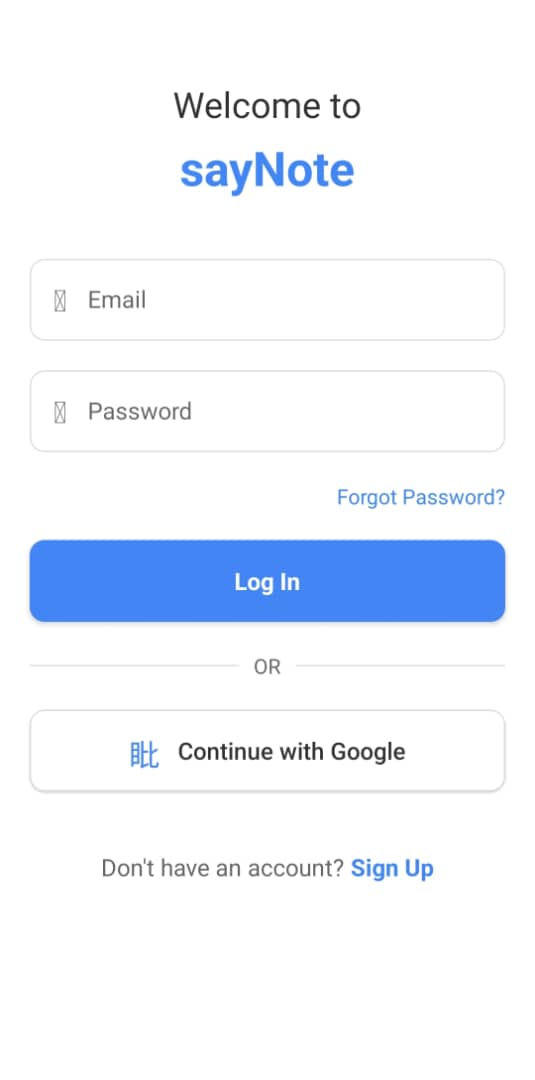
\includegraphics[width=0.4\textwidth]{assets/docs/mobile/login-page.jpeg}
    \hfill
    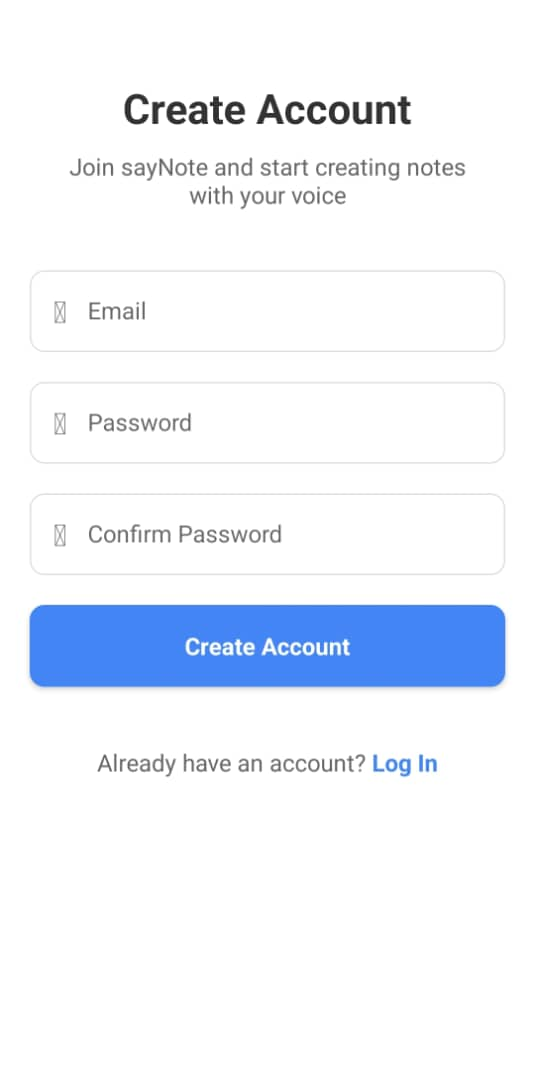
\includegraphics[width=0.4\textwidth]{assets/docs/mobile/create-account-page.jpeg}
    \caption{Écrans de connexion et de création de compte}
    \label{fig:mobile-auth}
\end{figure}

\begin{figure}[H]
    \centering
    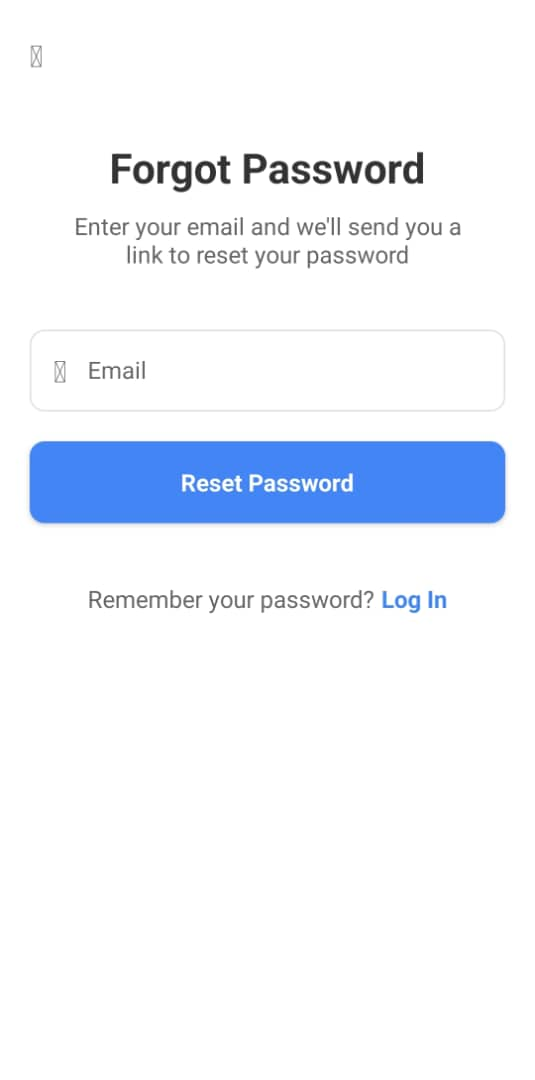
\includegraphics[width=0.4\textwidth]{assets/docs/mobile/forget-password-page.jpeg}
    \caption{Écran de réinitialisation du mot de passe}
    \label{fig:mobile-forgot-password}
\end{figure}

\subsubsection{Navigation et recherche}
\begin{figure}[H]
    \centering
    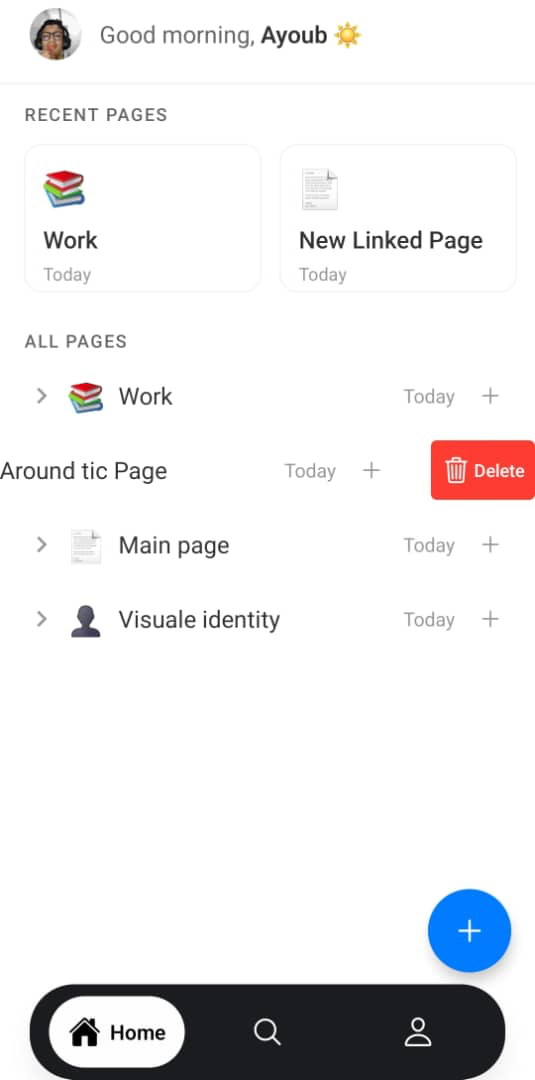
\includegraphics[width=0.4\textwidth]{assets/docs/mobile/home-screen.png}
    \hfill
    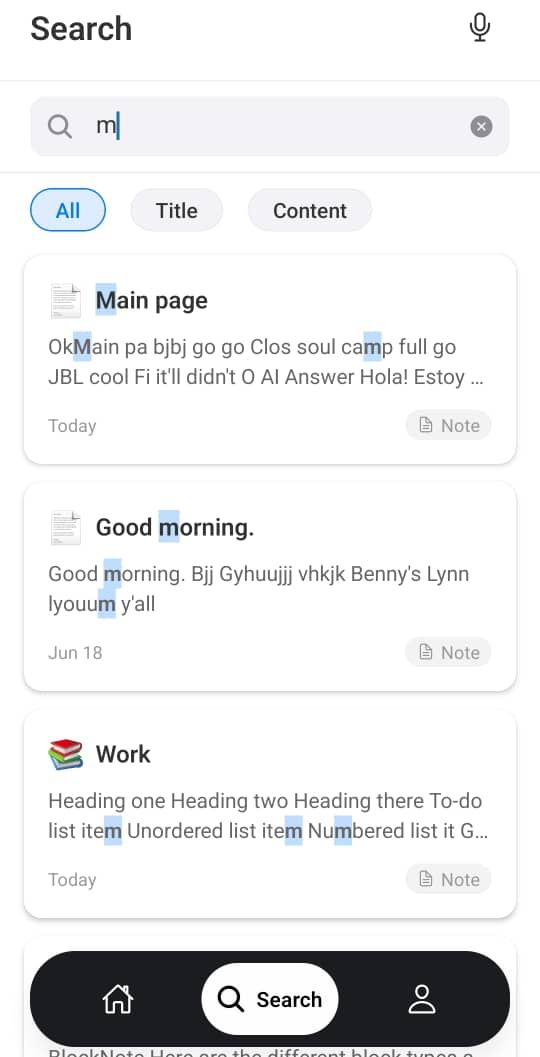
\includegraphics[width=0.4\textwidth]{assets/docs/mobile/search-screeen.png}
    \caption{Écrans d'accueil et de recherche}
    \label{fig:mobile-home-search}
\end{figure}

\subsubsection{Gestion des notes}
\begin{figure}[H]
    \centering
    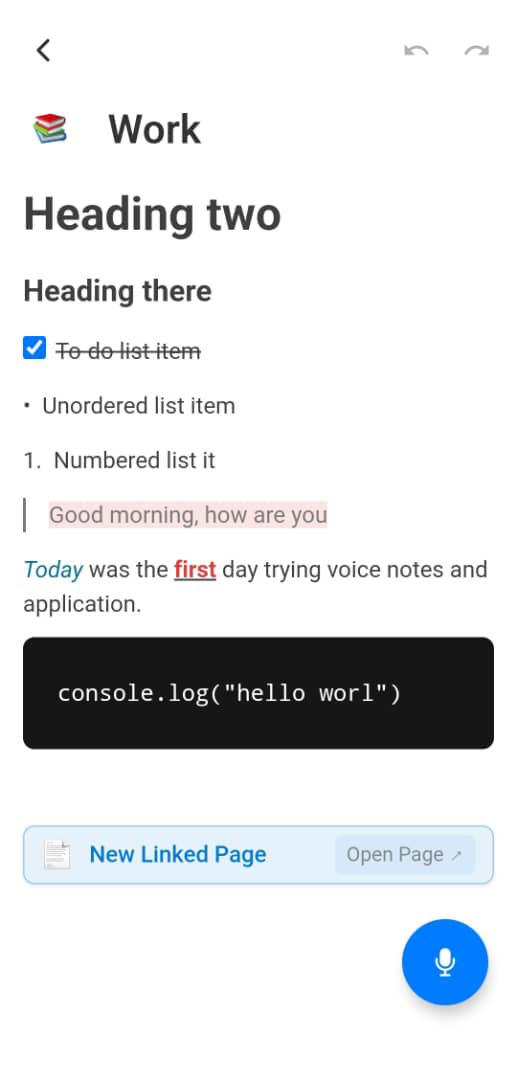
\includegraphics[width=0.4\textwidth]{assets/docs/mobile/note-page.png}
    \hfill
    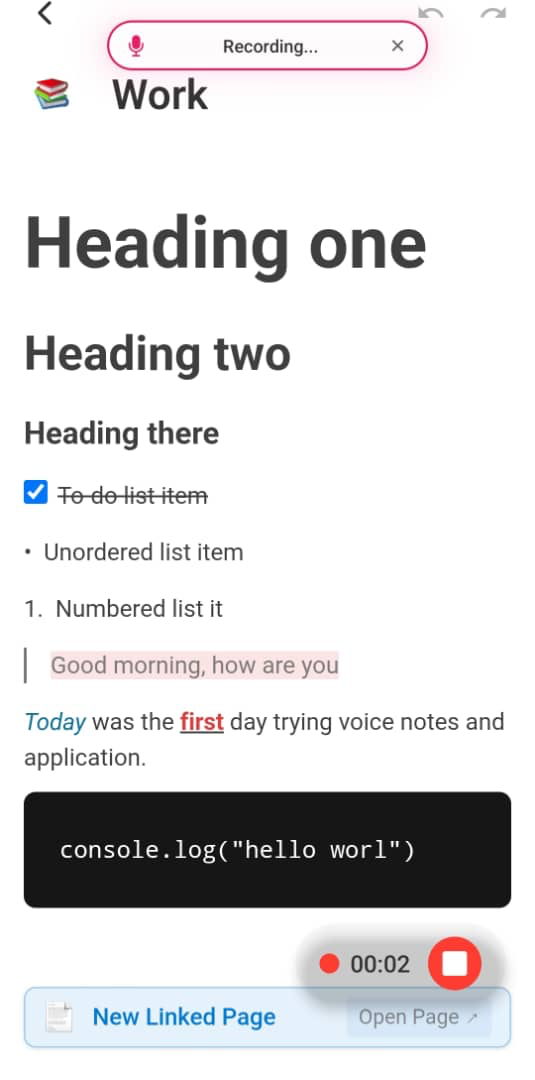
\includegraphics[width=0.4\textwidth]{assets/docs/mobile/note-page-recording.png}
    \caption{Éditeur de notes et enregistrement vocal}
    \label{fig:mobile-editor}
\end{figure}

\subsubsection{Profil utilisateur}
\begin{figure}[H]
    \centering
    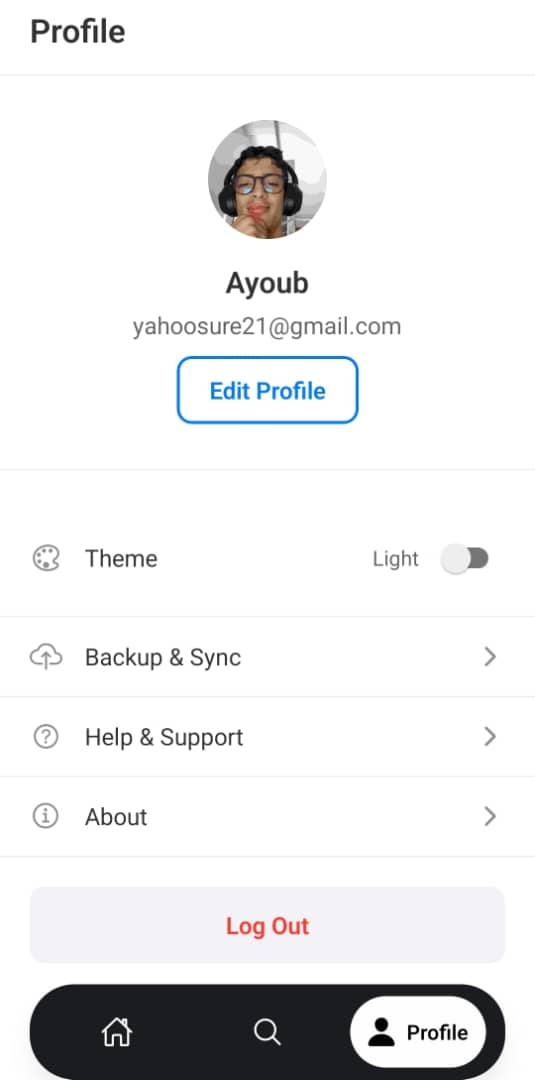
\includegraphics[width=0.4\textwidth]{assets/docs/mobile/profile-screen.png}
    \caption{Écran de profil utilisateur}
    \label{fig:mobile-profile}
\end{figure}

\section{Integration de la reconnaissance vocale}
\subsection{Gemini API}
\begin{minipage}{0.7\textwidth}
L'API Gemini de Google est un modele d'IA multimodal avance qui nous permet d'integrer des capacites de traitement du langage naturel et de comprehension contextuelle dans VoiceNotion. 

Cette API est au coeur de notre fonctionnalite de reconnaissance vocale et nous l'utilisons pour deux fonctions principales:
\begin{itemize}
    \item \textbf{Transcription de la parole en texte (Speech-to-Text)}: Conversion precise de l'audio vocal en texte ecrit
    \item \textbf{Analyse d'intention}: Comprehension et interpretation des commandes vocales pour executer les actions appropriees dans l'application
\end{itemize}

Gemini nous offre plusieurs avantages cles:
\begin{itemize}
    \item \textbf{Comprehension contextuelle}: Capacite a comprendre le contexte des commandes vocales
    \item \textbf{Support multilingue}: Prise en charge de multiples langues pour une utilisation internationale
    \item \textbf{Adaptabilite}: Possibilite d'affiner le modele pour notre cas d'utilisation specifique
    \item \textbf{Integration simple}: API REST facile a integrer dans nos applications web et mobile
\end{itemize}

Grace a Gemini, VoiceNotion peut offrir une experience de dictee vocale naturelle et intuitive, permettant aux utilisateurs de creer et de modifier du contenu a l'aide de commandes vocales complexes.
\end{minipage}%
\hfill
\begin{minipage}{0.25\textwidth}
\centering

\includegraphics[width=0.9\textwidth]{assets/docs/gemini.png}
\end{minipage}

\begin{figure}[H]
\centering
\textit{Image manquante: Diagramme de l'API Gemini}
\caption{Integration de l'API Gemini dans VoiceNotion}
\label{fig:gemini-api}
\end{figure}

\subsection{Flux de traitement des commandes vocales}
Le traitement des commandes vocales dans VoiceNotion suit un flux bien defini:
\begin{enumerate}
    \item Capture de l'audio via le microphone de l'appareil
    \item Conversion de l'audio en texte via l'API Gemini
    \item Analyse de l'intention de la commande (egalement via Gemini)
    \item Execution de l'action correspondante dans l'editeur
    \item Retour visuel et auditif a l'utilisateur
\end{enumerate}

\begin{figure}[H]
\centering
\textit{Image manquante: Flux des commandes vocales}
\caption{Flux de traitement des commandes vocales}
\label{fig:voice-commands-flow}
\end{figure}

\section{Tests et assurance qualite}
\subsection{Strategie de test}
Notre strategie de test pour VoiceNotion comprend plusieurs niveaux:
\begin{itemize}
    \item \textbf{Tests unitaires}: Verification du comportement des composants individuels
    \item \textbf{Tests d'integration}: Validation des interactions entre les differentes parties du systeme
    \item \textbf{Tests end-to-end}: Simulation des parcours utilisateur complets
    \item \textbf{Tests de performance}: Evaluation des temps de reponse et de la consommation de ressources
    \item \textbf{Tests d'accessibilite}: Verification de la conformite aux standards WCAG
\end{itemize}

\subsection{Outils de test}
\begin{itemize}
    \item \textbf{Jest}: Framework de test pour les tests unitaires et d'integration
    \item \textbf{React Testing Library}: Bibliotheque pour tester les composants React
    \item \textbf{Cypress}: Outil pour les tests end-to-end de l'application web
    \item \textbf{Detox}: Framework pour les tests end-to-end de l'application mobile
    \item \textbf{Lighthouse}: Outil pour evaluer les performances et l'accessibilite
\end{itemize}

\section{Deploiement et integration continue}
\subsection{Pipeline CI/CD}
Nous avons mis en place un pipeline d'integration continue et de deploiement continu (CI/CD) pour automatiser le processus de build, test et deploiement:

\begin{itemize}
    \item \textbf{GitHub Actions}: Automatisation des workflows de CI/CD
    \item \textbf{ESLint et Prettier}: Verification de la qualite du code
    \item \textbf{Tests automatises}: Execution des tests a chaque pull request
    \item \textbf{Preview Deployments}: Deploiement de versions de previsualisation pour chaque branche
\end{itemize}

\subsection{Environnements de deploiement}
\begin{itemize}
    \item \textbf{Developpement}: Environnement local pour les developpeurs
    \item \textbf{Staging}: Environnement de preproduction pour les tests
    \item \textbf{Production}: Environnement final accessible aux utilisateurs
\end{itemize}

\subsection{Plateformes de deploiement}
\subsubsection{Digital Ocean}
\begin{minipage}{0.7\textwidth}
Digital Ocean est une solution de service en cloud populaire, dotee d'une infrastructure robuste et offrant de multiples services.

Il est principalement utilise pour l'hebergement d'applications et de sites web et est prefere par les utilisateurs en raison de sa facilite d'utilisation. Les centres de donnees Digital Ocean offrent un haut niveau de securite pour les applications.

Les serveurs prives virtuels ou VPS offerts par Digital Ocean aux utilisateurs sont connus sous le nom de Droplets. Les utilisateurs de la plateforme peuvent gerer leurs applications par le biais d'une interface utilisateur Web ou d'une interface en ligne de commande (CLI).

La plateforme IaaS de Digital Ocean est un choix populaire pour de nombreuses grandes entreprises clientes dans le monde entier en raison de sa fiabilite. Elle permet aux utilisateurs de choisir des parametres tels que les centres de donnees pour les applications, la taille des droplets et la region geographique.

Pour VoiceNotion, nous avons utilise Digital Ocean pour:
\begin{itemize}
    \item Heberger notre base de donnees PostgreSQL de sauvegarde
    \item Gerer des services auxiliaires comme Redis pour la mise en cache
    \item Executer des taches de traitement en arriere-plan
\end{itemize}
\end{minipage}%
\hfill
\begin{minipage}{0.25\textwidth}
\centering
\textit{Logo DigitalOcean manquant}
\end{minipage}

\subsubsection{Nginx}
\begin{minipage}{0.7\textwidth}
Nginx, prononce comme "engine-ex", est un serveur web open-source qui, depuis son succes initial en tant que serveur web, est maintenant aussi utilise comme reverse proxy, cache HTTP, et load balancer.

Nginx a ete cree a l'origine par Igor Sysoev, avec sa premiere sortie publique en octobre 2004. Igor a d'abord concu le logiciel comme une reponse au probleme du C10k, qui est un probleme de performance lie a la gestion de 10.000 connexions simultanees.

Pour VoiceNotion, nous utilisons Nginx pour:
\begin{itemize}
    \item Servir de reverse proxy pour notre application
    \item Gerer le load balancing entre les instances de l'application
    \item Configurer le SSL/TLS pour la securite des communications
    \item Optimiser la diffusion des assets statiques
    \item Mettre en place des regles de cache pour ameliorer les performances
\end{itemize}

Nginx nous a permis d'ameliorer considerablement les performances et la securite de notre application, tout en offrant une flexibilite importante pour la configuration de notre infrastructure.
\end{minipage}%
\hfill
\begin{minipage}{0.25\textwidth}
\centering

\includegraphics[width=0.9\textwidth]{assets/docs/nginx.png}
\end{minipage}

\section{Securite et protection des donnees}
\subsection{Authentification et autorisation}
La securite de VoiceNotion repose sur plusieurs mecanismes:
\begin{itemize}
    \item \textbf{Authentification multi-facteurs}: Pour une securite renforcee des comptes
    \item \textbf{JWT (JSON Web Tokens)}: Pour la gestion des sessions
    \item \textbf{Controle d'acces base sur les roles}: Pour limiter les actions selon le profil utilisateur
\end{itemize}

\subsection{Protection des donnees}
\begin{itemize}
    \item \textbf{Chiffrement des donnees}: En transit (HTTPS) et au repos
    \item \textbf{Anonymisation}: Des donnees utilisees pour l'analyse et l'amelioration du service
    \item \textbf{Sauvegarde reguliere}: Pour prevenir la perte de donnees
\end{itemize}

\subsection{Conformite RGPD}
VoiceNotion est concu dans le respect du Reglement General sur la Protection des Donnees:
\begin{itemize}
    \item \textbf{Consentement explicite}: Pour la collecte et l'utilisation des donnees
    \item \textbf{Droit a l'oubli}: Possibilite de supprimer toutes les donnees utilisateur
    \item \textbf{Portabilite des donnees}: Export des notes dans des formats standards
\end{itemize}

\section{Defis techniques et solutions}
\subsection{Defis rencontres}
Durant le developpement de VoiceNotion, nous avons rencontre plusieurs defis techniques:
\begin{itemize}
    \item \textbf{Precision de la reconnaissance vocale}: Particulierement dans des environnements bruyants
    \item \textbf{Synchronisation en temps reel}: Entre les differents appareils d'un utilisateur
    \item \textbf{Performance de l'editeur}: Avec des documents volumineux
    \item \textbf{Fonctionnement hors ligne}: Gestion des conflits lors de la reconnexion
\end{itemize}

\subsection{Solutions implementees}
\begin{itemize}
    \item \textbf{Filtrage audio}: Algorithmes de reduction du bruit pour ameliorer la reconnaissance vocale
    \item \textbf{Systeme de replication}: Base sur CRDT (Conflict-free Replicated Data Types) pour la synchronisation
    \item \textbf{Virtualisation}: Rendu optimise des longs documents pour maintenir la performance
    \item \textbf{Queue de synchronisation}: Pour gerer les modifications hors ligne et les synchroniser lors de la reconnexion
\end{itemize}

\section{Conclusion}
L'implementation de VoiceNotion a necessite l'integration de nombreuses technologies modernes et la resolution de defis techniques complexes. L'architecture choisie nous a permis de creer une application performante, securisee et evolutive, disponible sur le web et sur mobile.

La combinaison de React, Next.js, React Native et Supabase nous a fourni une base solide pour construire notre solution, tandis que l'integration de l'API Gemini a rendu possible la fonctionnalite centrale de reconnaissance vocale.

Les prochaines etapes de developpement incluront l'amelioration continue de la precision de la reconnaissance vocale, l'ajout de nouvelles fonctionnalites collaboratives, et l'optimisation des performances sur tous les appareils. 